
% This LaTeX was auto-generated from an M-file by MATLAB.
% To make changes, update the M-file and republish this document.

\documentclass{article}
\usepackage{graphicx}
\usepackage{color}

\sloppy
\definecolor{lightgray}{gray}{0.5}
\setlength{\parindent}{0pt}

\begin{document}

    
    \begin{verbatim}
numRuns = 100;
theta = 1.0;
lambda = -100;
mu = 10;
Tmax = 0.1;
dt = 0.01;
T = linspace(0,Tmax,Tmax/dt);
X = zeros(numRuns,length(T));
dW = randn(numRuns,length(T));

for i = 1:numRuns
    X_j = 1.0;
    X(i,1) = X_j;
    for j = 2:length(T)
        X_j = (X_j + (1-theta)*lambda*dt*X_j + mu*sqrt(dt)*X_j*dW(i,j) + 0.5*mu*mu*dt*X_j*(dW(i,j)*dW(i,j) - 1))/(1-theta*lambda*dt);
        X(i,j) = X_j;
    end
end

plot(mean(X))
\end{verbatim}

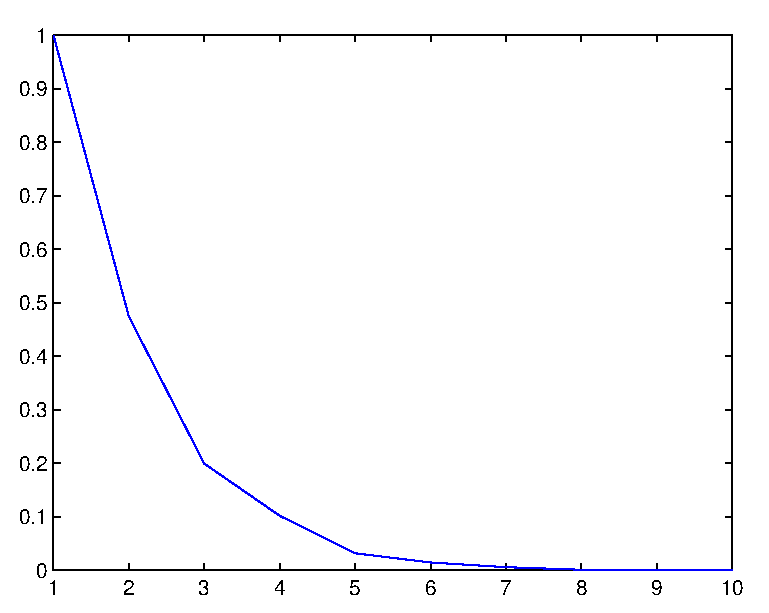
\includegraphics [width=4in]{q3_01.eps}



\end{document}
    
